\section{Sicherheit}

\paragraph{Angriffe}
\begin{items}
	\item Klassischer Angreifer (Dolev-Yao): Omnipräsent im Netz\\*
	- kann Pakete abhören / manipulieren / eigene Pakete erzeugen \\*
	- kein Zugriff auf Endsysteme\\*
	- keine Entschlüsselung ohne Schlüssel
	
	\item Abhören, Einfügen, Manipulieren, Man in the Middle, Replay, Denial of Service, 
	\item \( \leadsto \) \textbf{System/Protokoll} verwendet \textbf{Bausteine} um \textbf{Schutzziele} zu realisieren und vor \\* \phantom{.} \textbf{Angriffen} zu schützen
\end{items}

\paragraph{Schutzziele (CIA)}
\begin{items}
  \item \emph{Anforderungen an eine Komponente oder ein System, die erfüllt werden müssen, um schützenswerte Güter vor Bedrohen zu schützen}
  
  \medskip
  \item \textbf{\underline{C}onfidentiality} (Vertraulichkeit): keine unautorisierte Informationsgewinnung\\*
  	- Bausteine: Asymmetrische/Symmetrische Verschlüsselung
  	
  	\medskip
  \item \textbf{\underline{I}ntegrity} (Integrität): Kein Ersetzen, Einfügen oder Löschen von Daten \\*
  	- \textbf{starke Integrität}: Keine unautorisierte Manipulation von Daten möglich\\*
	- \textbf{schwache Integrität}: Manipulation von Daten nicht \emph{unbemerkt} möglich\\*
	- Manipulationen in vielen Fällen nicht zu verhindern \( \leadsto \) schwache Integrität\\*
  	- Bausteine: Tamper Proof-Module, Message Authentication Codes (MAC)
   
   \medskip
   \item \textbf{\underline{A}vailability} (Verfügbarkeit)\\*
     - \emph{Beschreibt, in welchem Maße die Systemfunktionalität von berechtigen Subjekten unabhängig von Einflüssen in Anspruch genommen werden kann}
   
   \medskip
   \item \textbf{Authentizität}\\*
     - \emph{Die angegebene Datenquelle ist tatsächliche Quelle} + Datenintegrität\\*
     - \textbf{Subjektechtheit}: Bob will sicherstellen, dass er tatsächlich mit Alice spricht \\* \( \leadsto \) \textbf{Authentifikation}\\*
     - \textbf{Datenechtheit}: Bob will sicherstellen, dass Daten tatsächlich von Alice sind\\*
     - Bausteine: Zertifikate, Signaturen, gemeinsames Geheimnis
     
     \medskip
  \item weitere Schutzziele: Privatheit, (Nicht-)Abstreitbarkeit
\end{items}

\paragraph{Verschlüsselung}
\begin{items}
	\item \textbf{symmetrisch}: Ent- und Verschlüsseln mit einem Schlüssel, sehr effizient
	\item \textbf{asymmetrisch}: Verschlüsseln: öffentlicher Schlüssel, Entschlüsseln: privater\\*
		Beispiel: RSA (Details: Siehe VL) % TODO
\end{items}

\paragraph{Kryptografische Hashfunktion}
\begin{items}
	\item Einwegfunktion ($H(m)$ effizient, $H^{-1}(c)$ nicht)
	\item Zu gegebenen $b$ schwierig, $a$ zu finden mit $H(a) = b$
	\item Schwache Kollisionsresistenz: Zu $a$ ein $a'$ mit $H(a) = H(a')$ schwer findbar
	\item Starke Kollisionsresistenz: Paar $a \neq a'$ mit $H(a) = H(a')$ schwer findbar
\end{items}

\paragraph{Integritätssicherung}
\begin{items}
	\item Daten sollen beim Empfänger genau so eintreffen, wie sie versendet wurden
	\item Manipulationen können nicht verhindert, nur erkannt werden -> Schwache Integrität
	\smallskip

	\item \textbf{Message Authentication Code}: \\*
		- Ziel: Empfänger erkennt Manipulation an empfangenen Daten \\*
		- Voraussetzung: Alice und Bob haben gleichen symmetrischen Schlüssel \\*
		- Vorgehensweise: Alice hängt Hash von (Nachricht + Schlüssel) an Nachricht an
		
		\smallskip
	\item \textbf{Digitale Signatur}: Sichert Integrität\\*
	- Ziel: Bob kann prüfen, dass wirklich Alice dieses Dokument unterschrieben hat \\*
	- Vorgehensweise: Hash des Dokuments mit privatem Schlüssel verschlüsseln, als \\* \phantom{-} Signatur mitsenden, entschlüsseln mit öffentlichem Schlüssel
	
	\smallskip
	\item \textbf{Digitales Zertifikat}: Sichert Authentizität\\*
	- Ziel: Verifizieren, dass jemand der ist, für den er sich ausgibt\\*
	 	(öffentlicher Schlüssel tatsächlich zu ihm gehört) \\*
	- Problem: kann man nicht selbst überprüfen \( \leadsto \) verlassen auf Dritte \\*
	- Vorgehensweise: Überprüfung durch \emph{certificate authority} (CA), \\* \phantom{-} ID-Zertifikat = Authentifikation des öffentlichen Schlüssels
\end{items}

\paragraph{E-Mail Sicherheit --- PGP (Pretty Good Privacy)}
\begin{items}
	\item SSL/TLS nur scheinbare Sicherheit: Weiterverarbeitung im Backend unverschlüsselt
	\item e-Mail Verschlüsselung mit PGP: Bietet Vertraulichkeit, Integrität und Authentizität
	\item Verwendet symmetrischen Schlüssel, der asymmetrisch Verschlüsselt zusammen mit Nachricht versendet wird
	
	\medskip
	\item Problem: Öffentliche Schlüssel müssen vor Versand bekannt sein
	\item Zugehörigkeit zur Mailadresse muss überprüfbar sein
	\item Bekanntgabe auf öffentlichen Schlüsselservern
	\item \textbf{Web of Trust}: Dezentraler, anarchischer Vertrauensansatz (ohne CAs)\\*
		- Transitive Überprüfung der Authentizität eines öffentlichen Schlüssels\\*
		- Nutzer bestimmt Vertrauens in die Signaturen anderer Nutzer (Signatory Trust)\\*
		- Key Legitimacy bestimmt sich aus Anzahl der vertrauten Signaturen
	\item In der Realität: Viele Probleme (Inseln)
\end{items}

\paragraph{Infrastruktursicherheit}
\begin{items}
	\item \textbf{Firewall}: Zugriffskontrolle durch Paketfilterung\\*
		- Teile des Netzes vor Eindringen unerwünschter Pakete schützen\\*
		- Netzbereiche (Intern, Internet, Demilitarized Zone) voneinander isolieren\\*
		- Zustandslos (IP, Port, Protokoll, Interface) mit Access Control List (ACL)\\*
		- Zustandsbehaftet (Überwacht TCP-Verbindungen)\\*
		- Application Layer Gateway: Filtern auf Basis von Nutzdaten (z.B. Username)
	\item \textbf{Intrusion Detection and Prevention}: \\*
		- Bekannte Angriffe erkennen / verhindern\\*
		- Deep Packet Inspection (Analyse der Nutzdaten)\\*
		- Anomaly Detection (Alarm bei Abweichungen vom Normalverhalten)
	\item \textbf{Organisatorische Maßnahmen}:\\*
		- Schulungen, Verantwortlicher, Notfallplan, Richtlinien, Datensicherung, \dots
\end{items}

%\paragraph{Sicherheitsprotokolle}
%\begin{items}
%	\item \textbf{System/Protokoll}: TLS/SSL, IPsec, Kerberos,...
%\end{items}
%\begin{figure}[H]\centering\label{Sicherheitsprotokolle}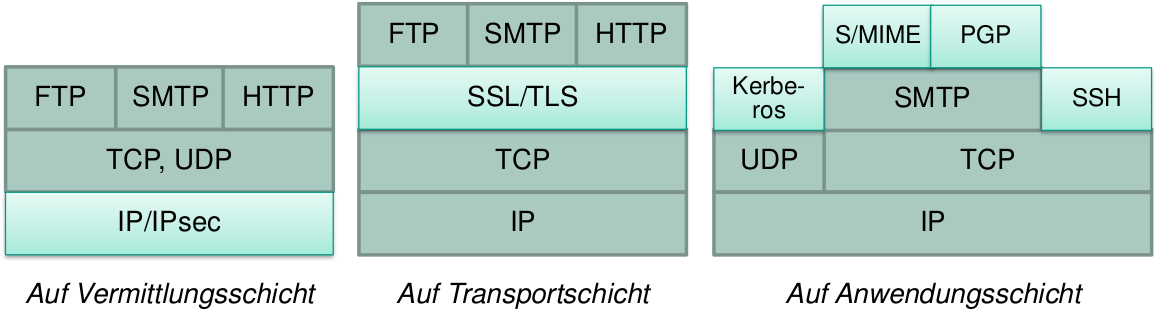
\includegraphics[width=0.33\textwidth]{Sicherheitsprotokolle}\end{figure}